\documentclass{standalone}
\usepackage{pgfplots}
\pgfplotsset{compat=1.18}

\begin{document}

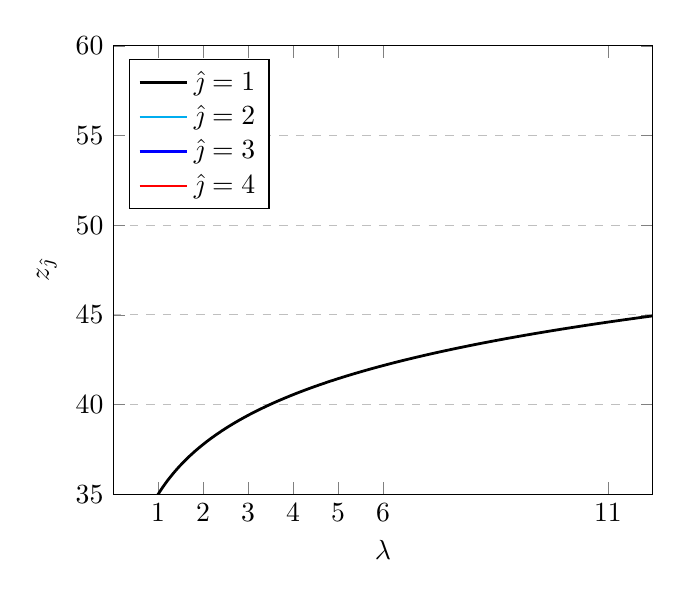
\begin{tikzpicture}
    \begin{axis}[
        title={},
        xlabel={$\lambda$},
        ylabel={$z_{\hat{\jmath}}$},
        xmin=0, xmax=12,
        ymin=35, ymax=60,
        xtick={1,2,3,4,5,6,11},
        ytick={35,40,45,50,55,60},
        legend pos=north west,
        ymajorgrids=true,
        grid style=dashed,
    ]
    
    % Line styles
    \addplot[
        domain=0:12, 
        samples=100,
        color=black,
        line width=1pt,
    ] {35 + 5 * ln(x) - 0.5 * ln(x^2)};
    \addlegendentry{$\hat{\jmath}=1$}
    
    \addplot[
        domain=0:12, 
        samples=100,
        color=cyan,
        line width=1pt,
    ] {-3.75 + 5 * ln(x) - 0.5 * ln(x^2)};
    \addlegendentry{$\hat{\jmath}=2$}
    
    \addplot[
        domain=0:12, 
        samples=100,
        color=blue,
        line width=1pt,
    ] {-7.5 + 5 * ln(x) - 0.5 * ln(x^2)};
    \addlegendentry{$\hat{\jmath}=3$}
    
    \addplot[
        domain=0:12, 
        samples=100,
        color=red,
        line width=1pt,
    ] {-11.25 + 5 * ln(x) - 0.5 * ln(x^2)};
    \addlegendentry{$\hat{\jmath}=4$}
    
    \end{axis}
\end{tikzpicture}

\caption{Schematic illustration of breakpoints. Each color depicts the objective function value when preserving a coordinate $\hat{\jmath}$, $z_{\hat{\jmath}}$, as a function of the penalty parameter $\lambda$.}
\label{fig:breakpoints}

\end{document}